
\chapter{Introdução}

\label{CapIntro}

% Resumo opcional. Comentar se não usar.
% \resumodocapitulo{Resumo opcional}


\section{RoboCup Soccer Simulation 2D}
\par A ideia de robôs jogando futebol foi proposta pela primeira vez em 1992 por Alan Mackworth\cite{mackworth1993seeing}.
Desde então a comunidade científica tem criado iniciativas buscando por soluções que tornem isso realidade.
Uma delas é a \textit{Robot World Cup Initiative}, abreviada como \textit{RoboCup}, que teve sua primeira edição em 1997 com mais de 40 equipes distribuídas entre as diversas categorias do evento.
\par O objetivo da iniciativa, definido pela \textit{RoboCup Federation}, é que por volta da metade do século XXI, um time de robôs humanóides autônomos vençam uma partida contra os campeões da Copa do Mundo mais recente. Mesmo que o objetivo pareça ambicioso, ele guia as pesquisas e motiva o avanço no campo.
Atualmente, a RoboCup conta com mais de 10 categorias, entre elas a \textit{RoboCup Soccer Simulation 2D}, abreviada RCSS, objeto de estudo deste projeto.
\par A categoria apresenta, também, grande relevância no cenário brasileiro.
Desde 2005, a RCSS está presente na maior competição de robótica da América Latina, a \textit{Latin American Robotics Competition}, LARC.
\par Nessa categoria, duas equipes de 11 jogadores autônomos e independentes jogam futebol em um ambiente virtual bidimensional.
Um servidor é responsável por esse ambiente e possui informação absoluta sobre o estado do jogo e suas regras.
Os jogadores, por sua vez, recebem dele informação incompleta e ruidosa de seus sensores virtuais, podendo executar comandos a fim de atuar sobre o estado do jogo.

\subsection{Servidor da partida}
\par Um servidor que executa a partida é disponibilizado pelos organizadores da competição e este pode ser utilizado, também, para desenvolvimento. O servidor, portanto, apresenta, internamente, algumas das regras da partida bem como um juiz autônomo que age para determinar gols, faltas e demais situações de uma partida de futebol. Caso necessário, um juiz humano poderá intervir em situações não contempladas pelas regras do servidor.
\par O servidor simula todos os movimentos e ações dos jogadores e da bola. Clientes externos se conectam ao servidor e cada cliente controla um único jogador. A comunição entre o cliente e o servidor é feita a partir do protocolo UDP por meio de mensagens com sintaxe específica e definida pelo servidor.
\par De forma a permitir o acompanhamento visual da partida, um monitor também é disponibilizado, porém não é necessário para que uma partida ocorra com sucesso.
\par O servidor, ainda, possui o modo \textit{trainer} para utilização durante treinamentos de algoritmos de inteligência computacional. Este modo permite a conexão de um cliente do tipo treinador que tem acesso absoluto às informações da partida e pode mudar modos de jogo e ainda mover arbitrariamente jogadores e bola. Adicionalmente, é possível acelerar os ciclos da partida permitindo o treinamento em tempo hábil.

\begin{figure}[h]
	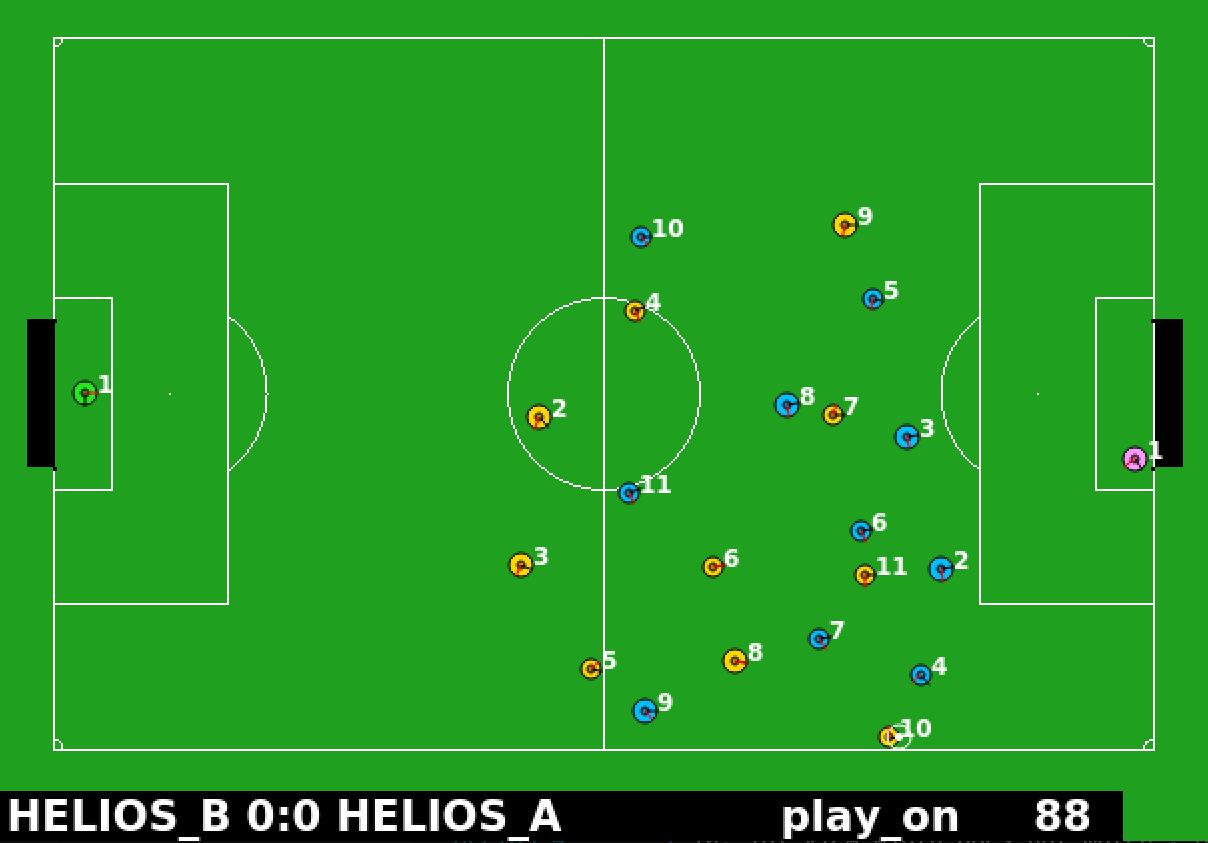
\includegraphics[width=0.7\linewidth]{figs/server.png}
	\centering
	\caption{Visualização de uma partida em andamento}
	\label{fig:rcssserver}
\end{figure}

\subsection{Cliente}
\par Os jogadores são controlados por clientes externos conectados ao servidor. Como já foi dito, um cliente corresponde a um único jogador e os clientes só podem ser comunicar com mensagens mandadas através do servidor da partida.
\par O cliente pode ser desenvolvido em qualquer linguagem desde que se comunique com o servidor pelo protocolo UDP e utilize a sintaxe de mensagens reconhecida pelo sistema. Há várias escolhas disponíveis para a construção do cliente, sendo decisão de cada equipe competidora como fazê-lo.

\begin{figure}[H]
	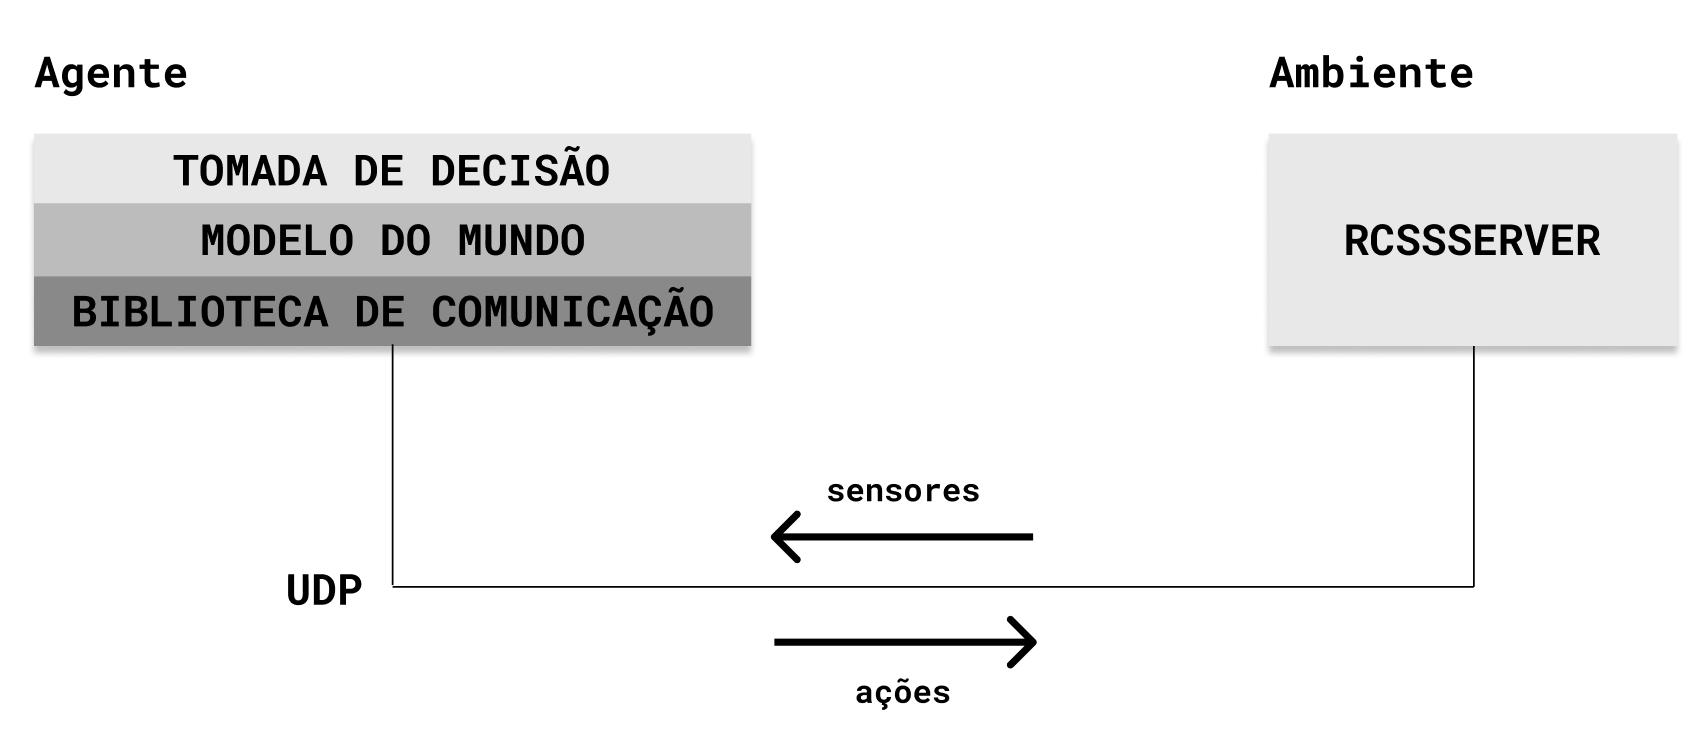
\includegraphics[width=0.9\linewidth]{figs/system.png}
	\centering
	\caption{Esquema ilustrando a arquitetura de um cliente e sua comunicação com o servidor do jogo.}
	\label{fig:system}
\end{figure}

\subsection{Sensores}

Para receber informações a respeito da situação do jogo, cada cliente conectado recebe mensagens referentes a atualizações de três sensores virtuais descritos abaixo.

\subsubsection{Sensor Auditivo}

As mensagens do sensor auditivo são do seguinte formato:

\textit{(hear Tempo Remetente "mensagem")}

Onde \textit{Tempo} é o número do ciclo em que a mensagem foi ouvida e \textit{Remetente} é descrição de quem enviou a mensagem. O \textit{Remetente} pode ser o árbitro, outros jogadores, um dos treinadores ou o próprio jogador.

No escopo deste trabalho, apenas as mensagens do árbitro serão consideradas, não sendo implementada nenhuma forma de comunicação direta entre os jogadores.

\subsubsection{Sensor Visual}

As mensagens do sensor visual contém as posições relativas referentes a cada objeto dentro do campo de visão do jogador. Esses objetos podem ser outros jogadores, marcadores como bandeiras e linhas (Figura \ref{fig:flags}) e a bola. O formato genérico é este:

\textit{(see (Objeto1)(Objeto2)(Objeto3)...(ObjetoN))}

Onde cada objeto tem o seguinte formato:

\textit{((NomeDoObjeto) Distância Direção VariaçãoDeDistância VariaçãoDeDireção DireçãoDoCorpo DireçãoDaCabeça)}

Sendo a distância e a direção dados em coordenadas polares, assim como suas variações. As informações de direção do corpo e da cabeça só aparecem quando o objeto em questão é um outro jogador.

\begin{figure}[H]
	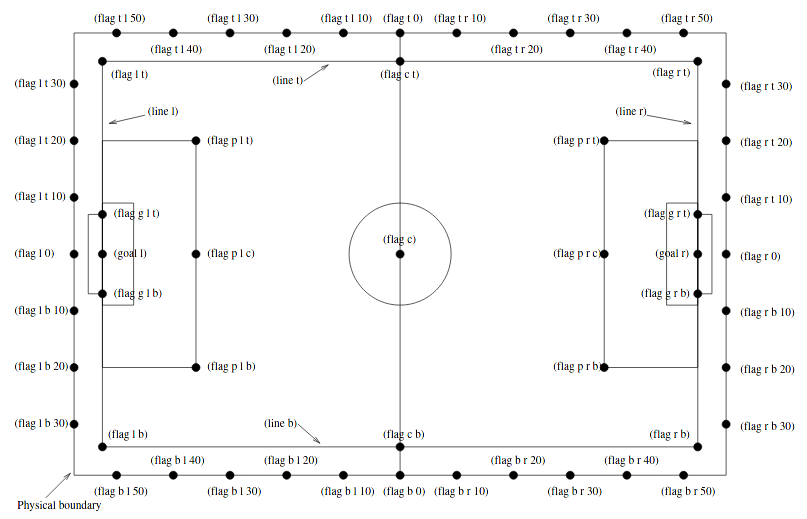
\includegraphics[width=0.9\linewidth]{figs/flags.png}
	\centering
	\caption{Indicadores espalhados pelo campo para que o agente possa estimar sua posição absoluta \cite{rcssmanual2003}.}
	\label{fig:flags}
\end{figure}

A riqueza de detalhes a respeito das informações obtidas depende da distância entre o objeto e o jogador. Por exemplo, caso esteja sendo visto outro jogador a uma distância muito grande, talvez seja impossível determinar o número de sua camisa ou até mesmo a qual time ele pertence. Em contrapartida, para jogadores próximos, é fornecido até mesmo a direção para a qual ele está olhando.

\subsubsection{Sensor Corporal}

O sensor corporal contém informações sobre o estado físico do jogador. Entre elas sua energia, que é consumida a cada ação tomada como chute ou arrancada (Seção \ref{sec:actions}), sua própria velocidade e direção de movimento, a direção de sua cabeça e a quantidade de cartões de advertência recebidos.

\subsection{Ações}
\label{sec:actions}

A cada ciclo de simulação, cada cliente conectado ao servidor pode realizar ações que terão efeito no ambiente. As ações são descritas abaixo. \cite{rcssmanual2003}

\subsubsection{Arrancar}
\label{sec:dash}

O comando de arrancar faz com que haja uma aceleração do jogador na direção da arrancada. Um parâmetro "potência" determina o valor da aceleração. É importante notar que o comando de arranque é o jeito padrão de movimentar um jogador.

Cada jogador possui uma certa quantidade de energia e o arranque tem um custo sobre ela. Ao começo de cada tempo da partida, a energia do jogador é colocada no máximo. Se o jogador acelera para frente, a energia é reduzida pelo valor de "potência". Se o jogador acelera para trás, o custo é maior e a energia é reduzida pelo dobro da potência.

Se a energia disponível é menor que a necessária para a realização com comando, o valor de "potência" é reduzido para que a quantidade necessária de energia seja a disponível.

\subsubsection{Chutar}

O comando de chute recebe dois parâmetros: a força e a direção do chute. Para realizar o comando, a bola precisa ser "chutável", ou seja, estar a uma certa distância do jogador.

Caso a bola não esteja diretamente à frente do jogador, a força efetiva será reduzida por um fator dependente da posição relativa da bola.

\subsubsection{Virar}

O comando virar recebe o momento angular a ser aplicado pelo jogador sobre si mesmo. Se o jogador não estiver em movimento, o seu ângulo é incrementado com o momento.

Porém, caso o jogador esteja em movimento, o resultado do comando é influenciado pelo momento de inércia do jogador (definido aleatoriamente pelo servidor no início da partida) e sua velocidade linear.

\subsubsection{Virar pescoço}

O jogador pode virar seu pescoço de maneira semi-independente de seu corpo. O ângulo do pescoço é relativo ao ângulo do corpo, então caso um comando virar seja executado, o ângulo absoluto do pescoço também mudará. Os ângulos máximo e mínimo em relação ao corpo são definidos na configuração do servidor, sendo o padrão +90 e -90 graus, respectivamente.

\subsubsection{Mover-se}
\label{sec:move}

O comando "mover-se" é utilizado para mover diretamente jogadores para coordenadas. Não pode ser utilizado no decorrer de uma partida, exceto quando o goleiro tem a posse da bola.  O comando fica disponível no início dos tempos da partida para posicionamento dos jogadores.

Para movimentar o jogadores durante a partida, o arranque Seção \ref{sec:dash}) deve ser utilizado.

\subsubsection{Agarrar}

O único jogador com permissão para agarrar ou pegar a bola é o goleiro. O goleiro pode pegar a bola em qualquer direção, desde que ela esteja dentro da área agarrável (Figura \ref{fig:catch}), definida como um retângulo com comprimento 2.0 e largura 1.0 na direção em que se deseja tentar agarrar.

Se o comando de agarrar falhar o goleiro fica incapacitado de agarrar a bola durante um número pré-determinados de ciclos do jogo. Se o comando tiver sucesso o goleiro pode usar o comando "mover-se" (Seção \ref{sec:move}) para se mover segurando a bola até um limite máximo de vezes estabelecido nas configurações do servidor.

\begin{figure}[H]
	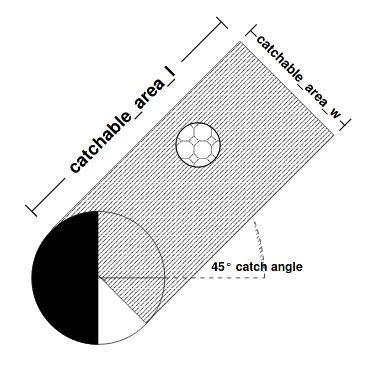
\includegraphics[width=0.5\linewidth]{figs/catch.png}
	\centering
	\caption{Visualização da área agarrável pelo goleiro \cite{rcssmanual2003}.}
	\label{fig:catch}
\end{figure}

\subsubsection{Falar}

Usado para transmitir mensagens aos outros jogadores. As mensagens devem ter comprimento menor que um valor pré-determinado pelo servidor. Os jogadores que estiverem à distância audível da mensagem receberão a mensagem do servidor imediatamente.

Como já dito, não será implementada nenhuma comunicação entre os jogadores neste trabalho.

\section{Abordagens utilizadas na categoria}
\par Uma pesquisa sobre as abordagens para o desenvolvimento das estratégias dos times participantes da RCSS revelou o uso recorrente de métodos de inteligência computacional.
\par A equipe chinesa \textit{WrightEagle}, campeã do principal evento internacional da categoria diversas vezes, utiliza Processos de Decisão de Markov ou MDPs para modelar a partida\cite{bai2015online}.
\par A equipe japonesa \textit{HELIOS}, campeã de 2018 da categoria na RoboCup, divide seus jogadores em categorias "chutadores" e "não-chutadores".
Os chutadores são responsáveis por realizar o planejamento de sequência de ações, utilizando métodos de valor de ação.
Os não-chutadores, por sua vez, não tem conhecimento do planejamento feito pelos chutadores, e devem obter o máximo de informações relevantes para tentar gerar a mesma sequência de ações que jogador chutador\cite{nakashima2018helios2018}.
\par A equipe brasileira \textit{ITAndroids}, atual campeã da LARC, utiliza a abordagem de sequência de ações, similar à \textit{HELIOS}, explorando uma árvore de ações criada dinamicamente de forma a maximizar o valor de cada ação. Além disso, utilizam Otimização por Enxame de Partículas \cite{melloitandroids} para adequar os parâmetros que calculam o valor da ação. A \textit{ITAndroids} também vem desenvolvendo o uso de Aprendizagem por Reforço Profunda \cite{maximoitandroids}.
\par Muitas equipes, ainda, desenvolvem seus agentes utilizando o agente base da equipe \textit{HELIOS}, \textit{Agent2d} com a biblioteca \textit{Librcsc}, escritas em C++. Por isso, é comum que haja semelhança na construção dos agentes dessas equipes.
